\section{Details for Benchmark Curation}
\label{appendix:benchmark}
% \pfliu{It would be nice, if we can introduce our benchmark design philosophy or principles, before describing actual details. See section 2 in \url{https://aclanthology.org/2023.emnlp-main.875.pdf}}

% \begin{table}[]
%     \centering
%     \renewcommand{\arraystretch}{1.5}
%     \caption{Statistics of the RAG benchmark. This benchmark is repurposed from  public datasets across 10 domains, containing 4,182 questions. For the domains of Finance, Lifestyle, Recreation, Technology, Science and Novel, the short answers are extended to long-form answers with GPT-4.}
%     \label{tab:benchmark_stat}
%     \scalebox{0.85}{
%     \begin{tabular}{>{\centering\arraybackslash}m{2cm}
%     >{\centering\arraybackslash}m{1.5cm}
%     >{\centering\arraybackslash}m{1.2cm}
%     >{\centering\arraybackslash}m{1.5cm}
%     >{\centering\arraybackslash}m{1.5cm}
%     >{\centering\arraybackslash}m{6cm}}
% \toprule
% Dataset & Domain & \# Query & \# Doc. & Source & Example Query \\
% \hline
% ClapNQ & Wikipedia & 300 & 4,293 & CLAPNQ & Difference between russian blue and british blue cat \\\hline
% NovelQA & Novel & 300 & 20 & NovelQA & When do the Ewell kids go to school? \\\hline
% RobustQA Writing & Writing & 500 & 199,994 & LoTTE, RobustQA & What is the difference between online and internet? \\\hline
% RobustQA BioASQ & Biomedical & 511 & 197,816 & BioASQ & What hand deformities do patients with Apert syndrome present with? \\\hline
% RobustQA Finance & Finance & 500 & 57,638 & FiQA, RobustQA & Is it safer to send credit card number via unsecured website form or by e-mail? What safer options are there? \\\hline
% RobustQA Lifestyle & Lifestyle & 500 & 119,461 & LoTTE, RobustQA & Can i eat a day old peanut butter sandwich? \\\hline
% RobustQA Recreation & Recreation & 500 & 166,975 & LoTTE, RobustQA & Why are so many american (spy) movies set in europe? \\\hline
% RobustQA Science & Science & 500 & 125,368 & LoTTE, RobustQA & Where is the flaw in this proof that 1=2? (derivative of repeated addition) \\\hline
% RobustQA Technology & Technology & 500 & 638,509 & LoTTE, RobustQA & Why not use larger cipher keys? \\\hline
% KIWI & AI Science & 71 & 429 & KIWI & What are the prior approaches proposed to improve faithfulness of the reasoning steps generated by LLMs and what tasks are they applied on? \\
% \bottomrule
%     \end{tabular}
%     }
% \label{tab:datasets}
% \end{table}

In this section, we introduce the benchmark datasets and the curation process for RAG evaluation. This benchmark datasets are derived from existing open-domain question answering (ODQA) datasets, including RobustQA~\cite{Han2023}, KIWI~\cite{xu2024kiwi}, ClapNQ~\cite{rosenthal2024clapnq}, and NovelQA~\cite{wang2024novelqa}. However, most of the ground truth answers in existing ODQA datasets are short answers, while the answers provided by modern LLM-based RAG systems tend to be long-form answers. Therefore, we repurpose the ODQA datasets by eliminating overly simple questions and converting the short answers into long-form answers to match the capabilities of current RAG systems. The statistics of the benchmark are summarized in Tab.~\ref{tab:benchmark_stat}. In the rest of this section, we describe the datasets we use and the curation process for each domain.


\subsection{Data Sources}

\paragraph{RobustQA}
We choose 7 domains from RobustQA's collection of datasets: Biomedical, Finance, Lifestyle, Recreation, Technology, Science, and Writing. For the Biomedical domain, following RobustQA, we employ the BioASQ~\cite{tsatsaronis2015overview} dataset, which contains human expert-written question-answer pairs and ground truth documents based on abstracts of articles from PubMed. We use the test sets for Task b from 2014 to 2023 and the corpus of v.2022 to construct the benchmark. We keep QA pairs whose answers are relatively long (more than 50 words), obtaining 511 QA pairs for the biomedical domain. The other 6 domains are sourced from FiQA~\cite{maia201818} and LoTTE~\cite{santhanam-etal-2022-colbertv2}, each of their question is annotated with a list of short answers that are spans of ground truth passages. We convert the short answers to long-form answers using GPT-4 and only keep the generated answers with no hallucinations, as checked by RefChecker. Finally, we sample 500 examples for each domain.


\paragraph{ClapNQ}
Derived from NaturalQuestions (NQ)~\cite{kwiatkowski-etal-2019-natural}, an ODQA dataset based on Wikipedia, ClapNQ has long-form answers annotated for a subset of NQ for evaluating RAG. We employ the dev set of ClapNQ in our benchmark and take the annotated long-form answers as the ground truth.


\paragraph{KIWI}
is constructed by asking LLMs research questions about a set of NLP papers and guiding the LLMs to reach satisfactory long-form answers. The authors validated the quality of the generated answers by rating them as ``good'', ``neutral'', or ``bad''. We take the answers labeled ``good'' as the ground truth answers and query the full text of the papers from S2ORC~\cite{lo-etal-2020-s2orc} as the corpus. As a result, we obtain 71 QA pairs and 429 papers as the corpus.

\paragraph{NovelQA}
is a benchmark for question answering over long novels containing over 100K tokens on average. Originally designed for benchmarking long-context LLMs, we repurpose it for evaluating RAG. In contrast with the other domains, each question in NovelQA is associated with a single novel, so when we use this dataset for RAG, we constrain the retrieval to within the corresponding novel. We select 19 copyright-free novels and convert the corresponding short answers to long-form answers following the same process for RobustQA.


\subsection{Long-form Answer Generation}

We employ GPT-4 (\texttt{gpt-4-turbo-2024-04-09}) to convert the human annotated short answers to long-form answers in the dataset of RobustQA and NovelQA. For RobustQA, the short answers are spans of the annotated ground truth passages, we take all the annotated short answers and the corresponding passages in the prompt and ask GPT-4 to convert them to one single long-form answer. For NovelQA, we take the human written evidences as the ground truth passage content and the human written short answers for the long-form answer generation. The prompt is shown in Fig.~\ref{fig:long_form_answer_prompt}.

For quality control, we ask GPT-4 to generate the passage IDs associated with the long-form answer. We use RefChecker to check whether all the claims of a long-form answer are entailed by these passages, and we only keep the long-form answers that meet this criteria. The RefChecker we used here are described in Appendix~\ref{appendix:refchecker_validation}.

\begin{figure}[h]
    \centering
    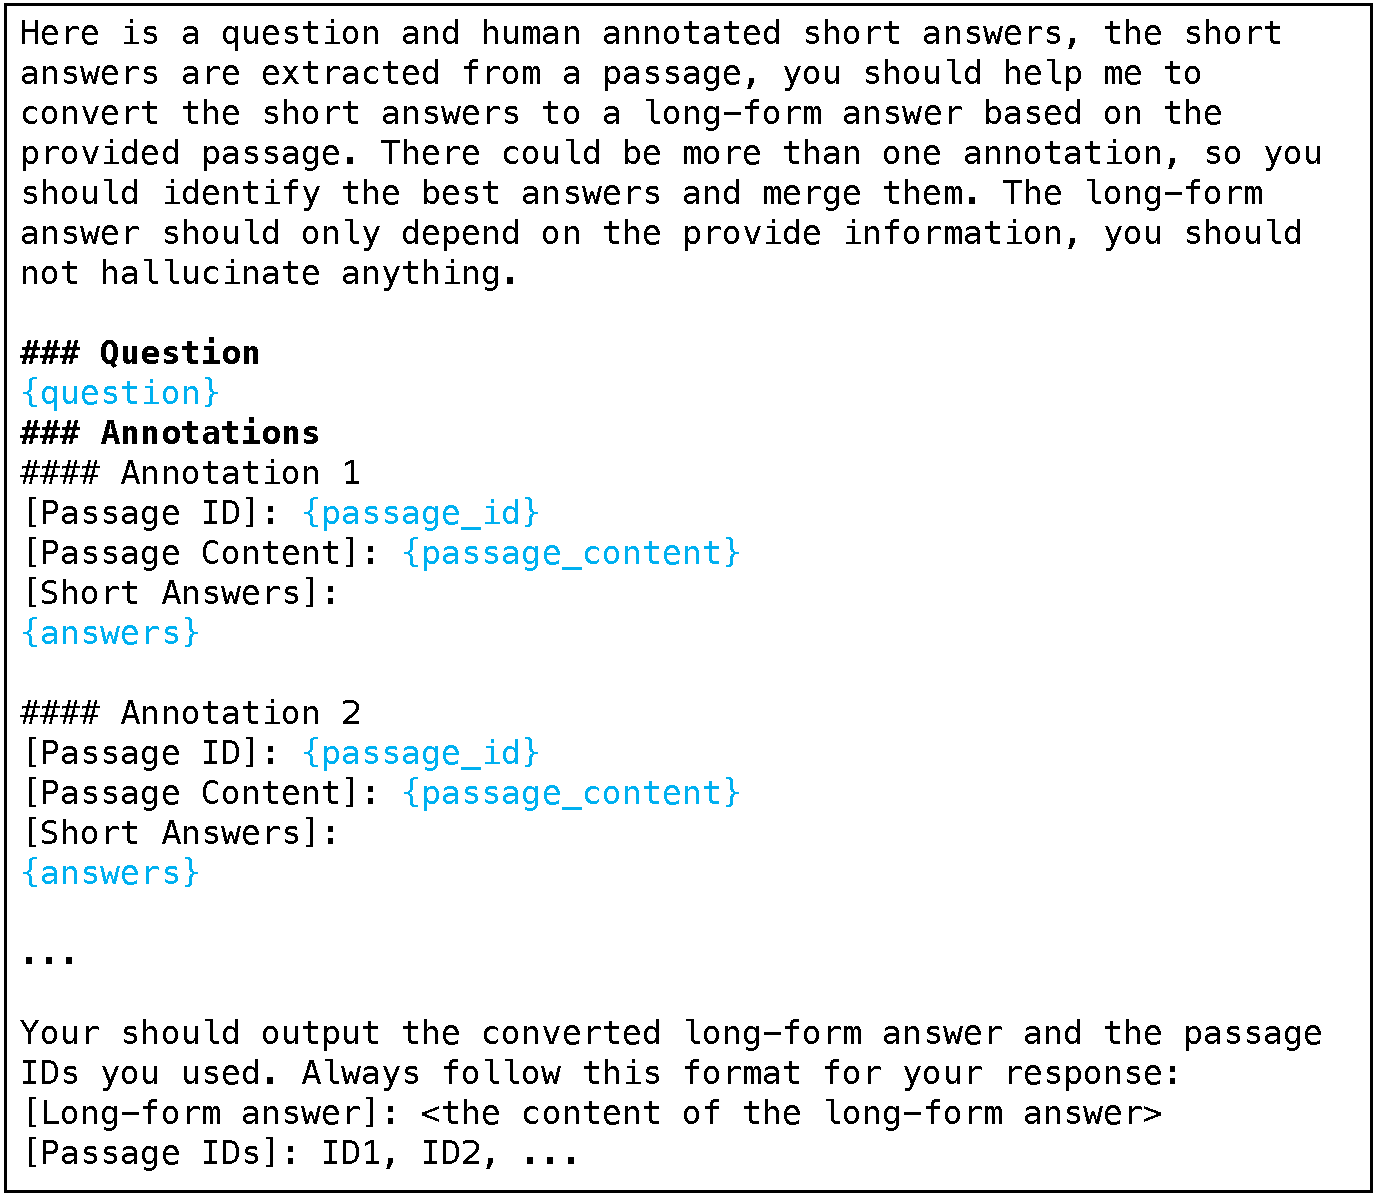
\includegraphics[width=0.8\textwidth]{figures/robustqa_longform_answer_generation_prompt.pdf}
    \caption{The prompt used for converting short answers to long-form answers for the domains of Novel, Finance, Lifestyle, Recreation, Technology, Science, and Writing.}
    \label{fig:long_form_answer_prompt}
\end{figure}

\subsection{Corpus Downsampling for Science and Biomedical Domains}

In addition to long-form answer generation, we also perform downsampling for the corpora of Science and Biomedical domains as they are much larger than the others, with over 1 million documents each. 
Building indexes for a dense retriever is very costly for large corpora, so we downsample these domains to lower the evaluation cost for the community.
For the biomedical domain, we first use BM25 retriever to obtain top 400 documents for each question. The subsampled corpus is formed by combining all documents from the retriever with annotated relevant documents from the datasets.
Based on our initial study, we observe that the BM25 retriever yeild competitive performance against the dense retriever, so we decide to only use the BM25 retriever for downsampling purpose to save compuation cost.
For the science domain, we leverage both the BM25 retriever and e5-mistral-7b-instruct based dense retriever to obtain document candidates.
Specifically, we retrieve the top 200 documents from both retrievers (400 documents in total before deduplication).
Similarly, the combination of all documents from the retrievers and annotated relevant documents from datasets forms the downsampled corpus.


\subsection{License of The Datasets}

The annotations from RobustQA, ClapNQ and NovelQA are under Apache-2.0 License. The corpora of Finance and annotations of KIWI are under CC-BY-SA-4.0. BioASQ is under CC BY 2.5 license. The license for the corpora of LoTTE are not specified.